\newpage
\section{Model-to-Tree transformation with TGGs}
\genHeader

One powerful benefit of working with TGG transformations is that by specifiying one transformation (i.e., a forward transformation), we're able to get the
opposite direction for free! Our example used a \texttt{tree.xmi} (\texttt{MocaTree}
instance) input, transformed it forward into \texttt{tree.xmi\_fwd.xmi} (\texttt{Dictionary} instance), and used that result file in a backwards
transformation to create the final tree output, \texttt{tree.xmi\_FWD.xmi\_BWD.xmi}, all without error! If our TGG was truly successful however,
the starting and final files should be identical. Let's compare the two (Fig.~\ref{eclipse:comparingTreeModels}).

\vspace{0.5cm}

\begin{figure}[htpb]
\begin{center}
  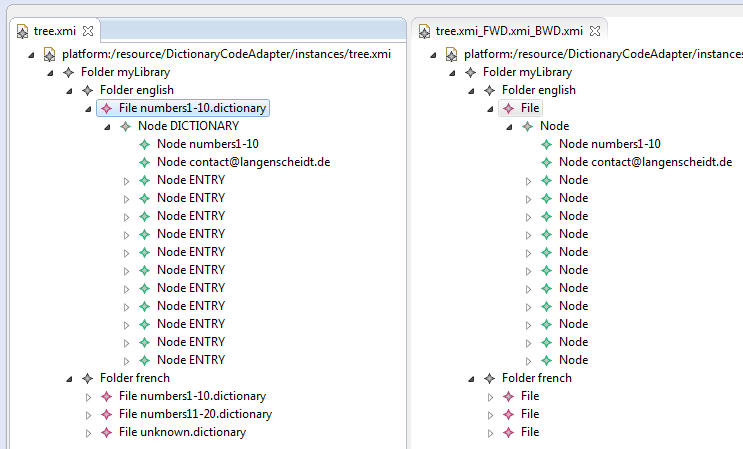
\includegraphics[width=\textwidth]{eclipse_generatedBackwardsModel}
  \caption{Not yet identical trees}
  \label{eclipse:comparingTreeModels}
\end{center}
\end{figure}

\vspace{0.5cm}

It's close, but not perfect. You can see that some things need to be refined. The ``DICTIONARY'' and ``ENTRY'' labels, for example, are missing from the
major nodes. We need to include an attribute constraint to bind these specific EString values. You'll also notice that, as you scroll through each
\texttt{Node}, the \texttt{title} and \texttt{author} nodes have the correct \texttt{index} values of 0 and 1, but the remaining \texttt{entry} indices are also
set to 0.
We were only concerned with binding the title and author nodes in the forward direction, as we could assume that any other node with any other index value (2 and greater) was an
\texttt{entryNode}. In the backwards direction however, this distinction is lost, which means we must introduce a custom attribute constraint.

\jumpDual{m2tvis}{m2ttex}

\newpage
\hypertarget{m2tvis}{}
\subsection{Double-checking the TGG}
\visHeader

\begin{itemize}

\item[$\blacktriangleright$] Open \texttt{NodeToDictionaryRule} and update as depicted below (via attribute constraint). Is this in the right place? Should this
be done before??

\begin{figure}[htp]
\begin{center}
  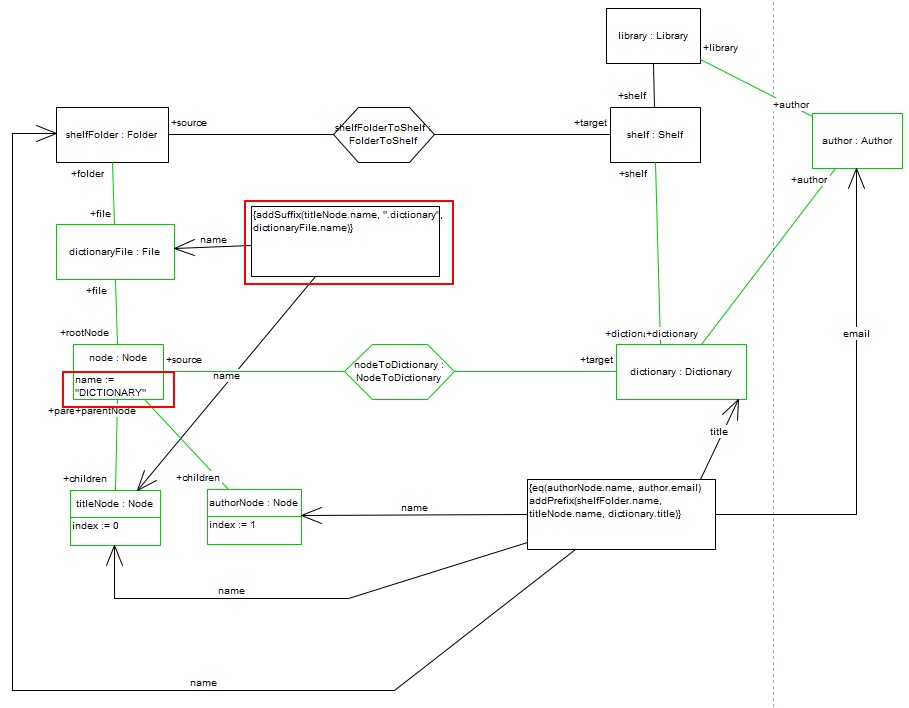
\includegraphics[width=\textwidth]{ea_updateNodeToDictionary}
  \caption{updated NodeToDictionary}
  \label{ea:NodeToDictionary_updated}
\end{center}
\end{figure}

\item[$\blacktriangleright$] Similarly, open \texttt{ForAllEntry} in EA and update like so:

\begin{figure}[htp]
\begin{center}
  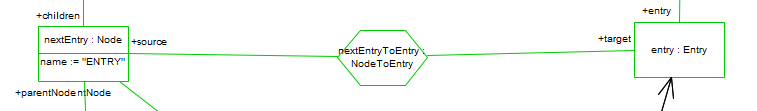
\includegraphics[width=\textwidth]{ea_updateForAllEntry}
  \caption{updated ForAllEntry}
  \label{ea:ForAllEntry_updated}
\end{center}
\end{figure}

\item[$\blacktriangleright$] End comment.

\jumpSingle{finalStep}

\end{itemize}


\newpage
\hypertarget{m2ttex}{}
\subsection{Refining the TGG Transformation}
\texHeader

\begin{itemize}

\item[$\blacktriangleright$] Find the relevant files and add the following attribute constraints. Note : the MOSL parser requires that all attribute constraints
are declared before link variables.

\begin{figure}[htp]
\begin{center}
  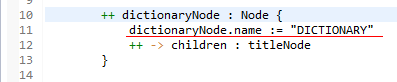
\includegraphics[width=0.8\textwidth]{eclipse_NodeToDictionaryRule_updated}
  \caption[labelInTOC]{needs refinement\ldots}
  \label{eclipse:generatedBkwrdMdl}
\end{center}
\end{figure}

\begin{figure}[htp]
\begin{center}
  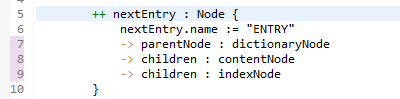
\includegraphics[width=0.8\textwidth]{eclipse_ForAllEntryRule_updated}
  \caption[labelInTOC]{needs refinement\ldots}
  \label{eclipse:generatedBkwrdMdl}
\end{center}
\end{figure} 

\item[$\blacktriangleright$] Add new SetDefaultNumber CSP here.

\begin{figure}[htbp]
\begin{center}
  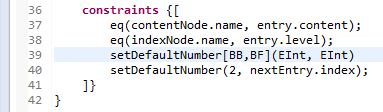
\includegraphics[width=0.6\textwidth]{eclipse_setDefaultNumberConstraint}
  \caption{extra constraint}
  \label{eclipse:newEntryConstraint}
\end{center}
\end{figure}

\end{itemize}


\newpage
\hypertarget{common cspConstraint}{}
\subsection{Implementing SetDefaultNumber}
\genHeader

\begin{itemize}

\item[$\blacktriangleright$]  Navigate and expand ``DictionaryCodeAdapter/src/csp.constraints.'' Open \texttt{SetDefaultNumber.java} and edit this file until it
matches Fig.~\ref{eclipse:setDefaultImpl}.

\vspace{0.5cm}

\begin{figure}[htbp]
\begin{center}
  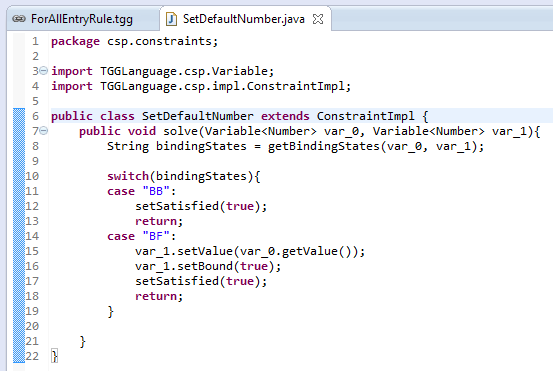
\includegraphics[width=0.9\textwidth]{eclipse_setDefaultNumberImplementation}
  \caption{Completing the custom \texttt{setDefaultNumber} constraint}
  \label{eclipse:setDefaultImpl}
\end{center}
\end{figure}

\item[$\blacktriangleright$] After saving, and run \texttt{TGGMain} one more time. The initial and final \texttt{tree} variants should now be nearly
identical! The only difference should be that, instead of each \texttt{entry.index} value increasing (as seen in \texttt{tree.xmi}), each value should now be
set to exactly 2. Their order may be different, depending on how the transformation processed them, but their \texttt{index} values should all  be correct.

\vspace{0.5cm}

\item[$\blacktriangleright$] Your transformation is nearly complete! The only remaining step is to unparse this final tree structure into an output filesystem.
Before we move on however, let's reflect on how easy and short it was to implement this `backwards' transformation. If we were to use another method (such as
SDMs), we would have had to create at least six more independent rules to handle this. Instead, TGGs gave us this direction for free!

\end{itemize}

